\clearpage
\section*{\currfilename}

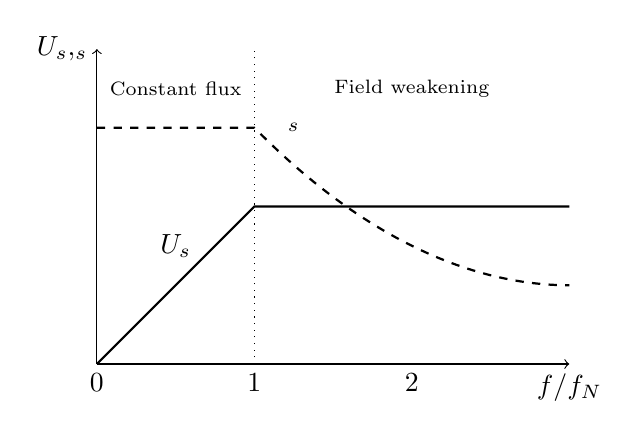
\begin{tikzpicture}
  % Horizontal axis
  \draw[->] (0,0) -- (6,0) node[anchor=north] {$f/f_N$};

  % Labels
  \draw (0,0) node[anchor=north] {0}
        (2,0) node[anchor=north] {1}
        (4,0) node[anchor=north] {2};

  % Ranges
  \draw (1,3.5) node{{\scriptsize Constant flux}}
        (4,3.5) node{{\scriptsize Field weakening}};

  % Vertical axis
  \draw[->] (0,0) -- (0,4) node[anchor=east] {$U_s,\varPsi_s$};

  % Nominal speed
  \draw[dotted] (2,0) -- (2,4);

  % Us
  \draw[thick] (0,0) -- (2,2) -- (6,2);
  \draw (1,1.5) node {$U_s$};
  % Psis
  \draw[thick,dashed] (0,3) -- (2,3) parabola[bend at end] (6,1);
  \draw (2.5,3) node {$\varPsi_s$};
\end{tikzpicture}
